% --- [ Control Flow Analysis Example ] ----------------------------------------

\subsection{Control Flow Analysis Example}
\label{app:control_flow_analysis_example}

This section provides a step-by-step demonstration of how the control flow analysis is conducted by analysing the \texttt{stmt} function of the c4\footnote{C in four functions: \url{https://github.com/rswier/c4}} compiler. For a detailed description of the control flow analysis stage, please refer to section \ref{sec:design_control_flow_analysis}. The control flow analysis operates exclusively on CFGs, which are generated by a set of components prior to the control flow analysis stage. Firstly, the C source code of the c4 compiler is translated into LLVM IR by the Clang compiler of the front-end. Secondly, the LLVM IR is optionally optimized by the \texttt{opt} tool of the LLVM compiler framework. Lastly, a CFG is generated for each function of the LLVM IR using the \texttt{ll2dot} tool. For this demonstration, the CFG of the \texttt{stmt} function is the starting point of the control flow analysis stage.

The first step of the control flow analysis recursively locates subgraph isomorphisms of the graph representation of pre-test loops (see figure \ref{fig:pre_loop_graph_representation}) in the original CFG of the \texttt{stmt} function, and replaces these subgraphs with single nodes as illustrated in figure \ref{fig:step_1}.

The second step further simplifies the CFG of \textbf{step 1} by recursively replacing the subgraph isomorphisms of the graph representation of consecutive statements (see figure \ref{fig:list_graph_representation}) with single nodes, as illustrated in figure \ref{fig:step_2}.

The third step further simplifies the CFG of \textbf{step 2} by recursively replacing the subgraph isomorphisms of the graph representation of 1-way conditionals (see figure \ref{fig:if_graph_representation}) with single nodes, as illustrated in figure \ref{fig:step_3}.

The fourth step further simplifies the CFG of \textbf{step 3} by recursively replacing the subgraph isomorphisms of the graph representation of 1-way conditionals with body return statements (see figure \ref{fig:if_return_graph_representation}) with single nodes, as illustrated in figure \ref{fig:step_4}.

The last step of the control flow analysis stage reduces the CFG of \textbf{step 4} into a single node by recursively replacing the subgraph isomorphisms of the graph representation of 2-way conditionals (see figure \ref{fig:if_else_graph_representation}) with single nodes, as illustrated in figure \ref{fig:step_5}.

When the CFG has been reduced into a single node, a structured CFG may be generated which maps each node to a high-level control flow primitive; as further described in appendix \ref{app:restructure_example}. Should the control flow analysis fail to reduce the CFG into a single node, the CFG is considered irreducible with regards to the supported high-level control flow primitives, a summary of which are presented in figure \ref{fig:graph_representations} of section \ref{sec:lit_review_control_flow_analysis}.

% pre_test
\begin{figure}[htbp]
	\centering
	\begin{subfigure}[ht]{0.45\textwidth}
		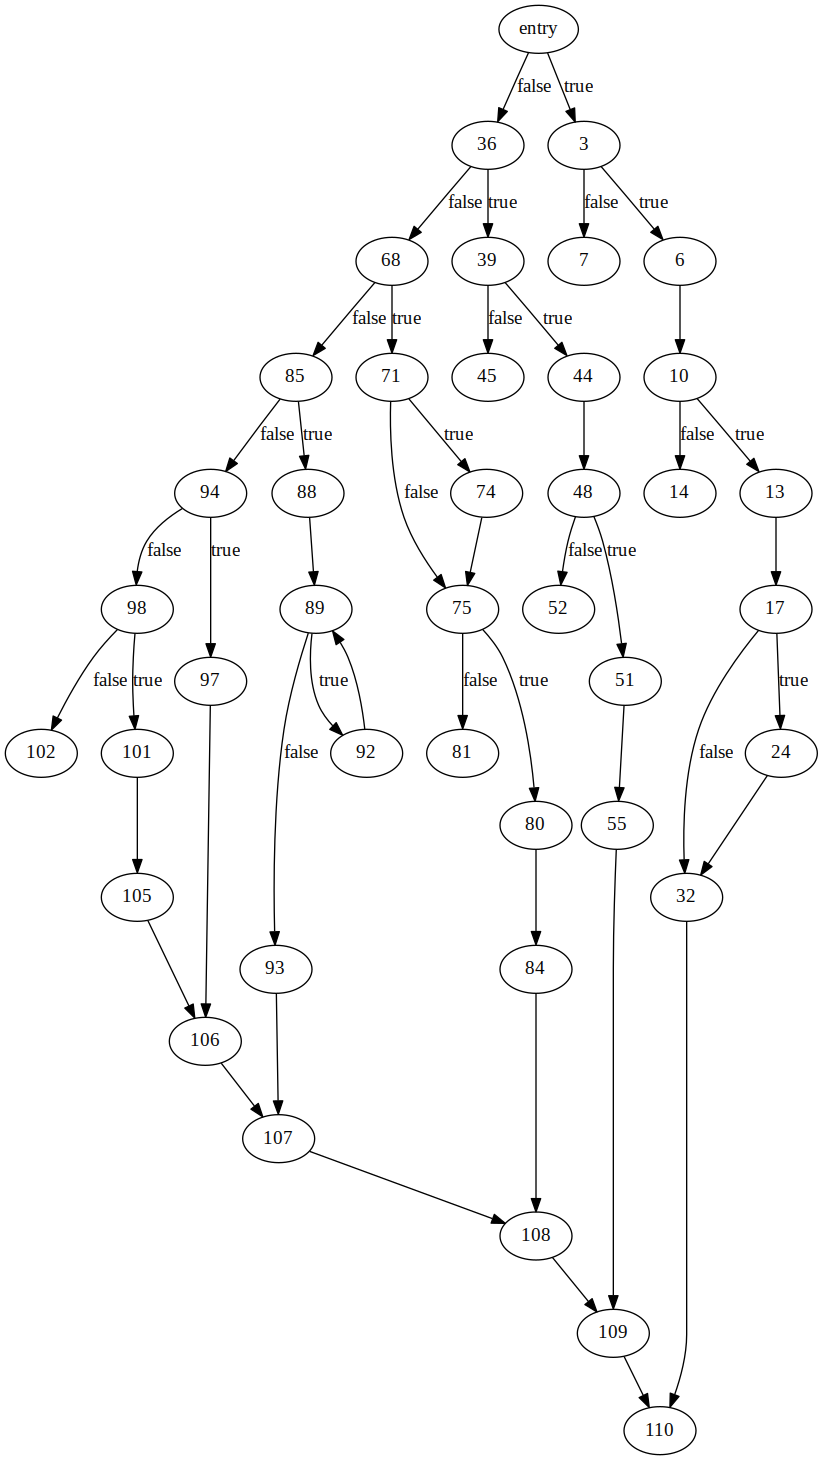
\includegraphics[width=\textwidth]{inc/appendices/control_flow_analysis_example/stmt_0.png}
	\end{subfigure}
	\qquad
	\begin{subfigure}[ht]{0.45\textwidth}
		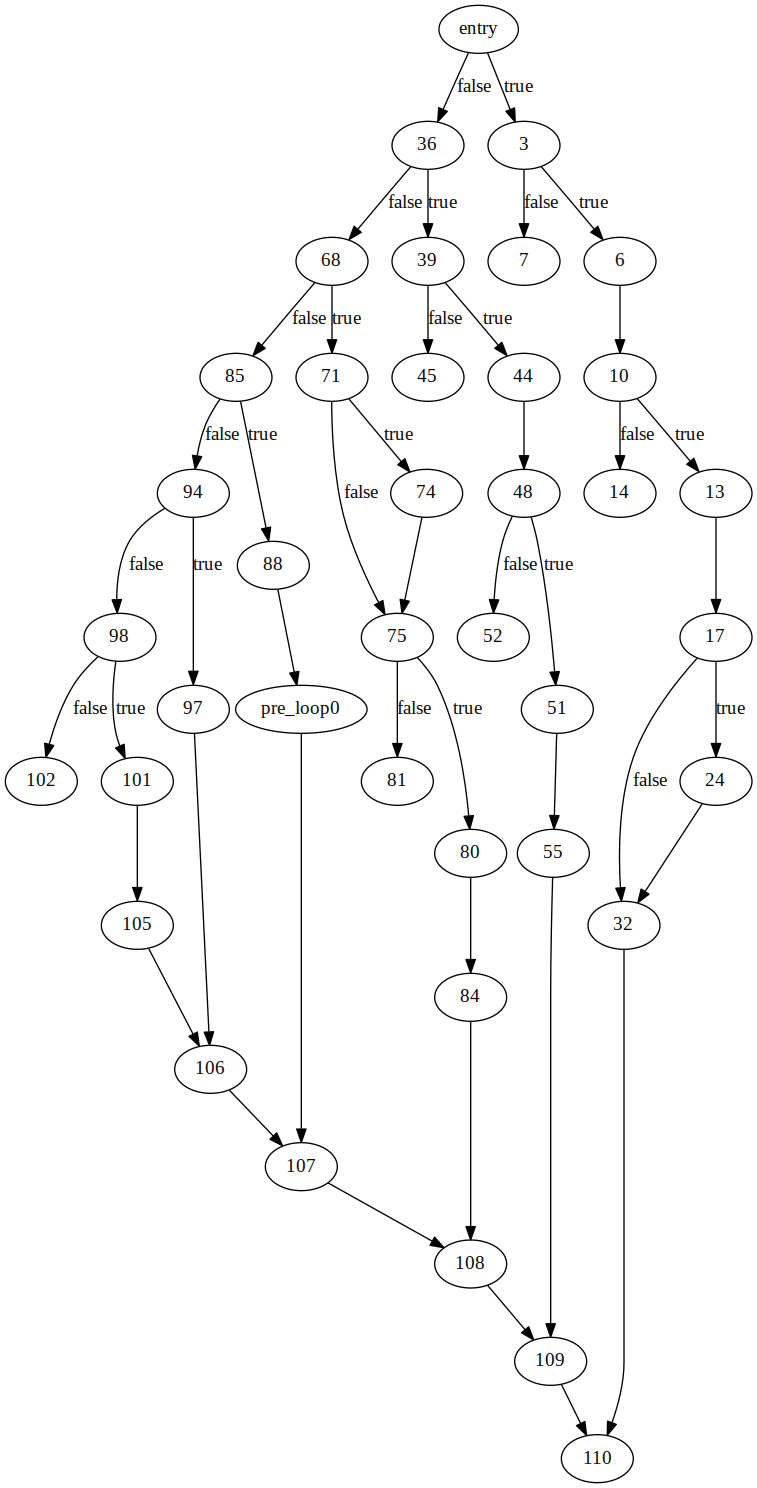
\includegraphics[width=\textwidth]{inc/appendices/control_flow_analysis_example/stmt_1.png}
	\end{subfigure}
	\caption{\textbf{Step 1}. The original CFG of the \texttt{stmt} function (left) and a simplified CFG (right) after identifying pre-test loops (see figure \ref{fig:pre_loop_graph_representation}).}
	\label{fig:step_1}
\end{figure}

% list
\begin{figure}[htbp]
	\centering
	\begin{subfigure}[ht]{0.45\textwidth}
		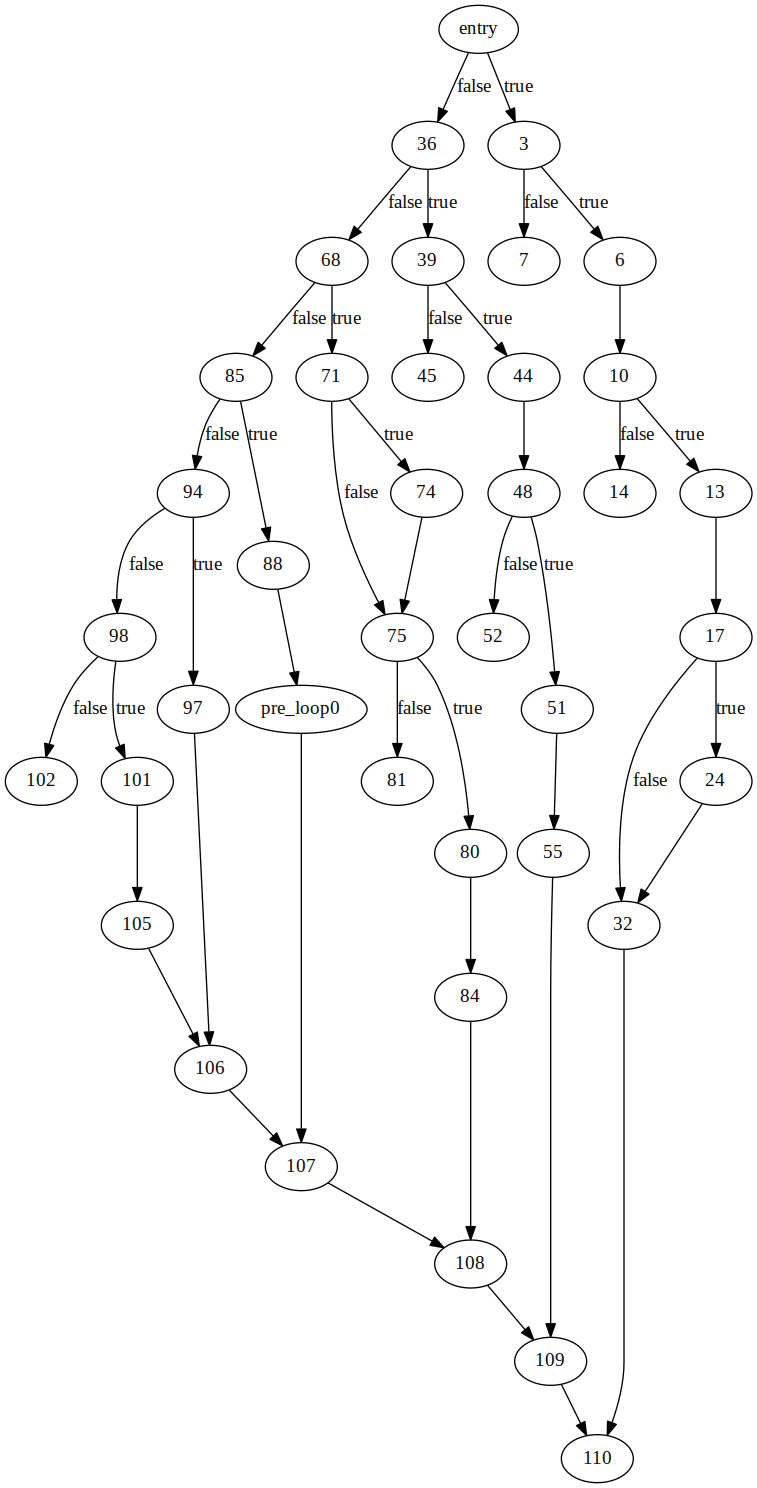
\includegraphics[width=\textwidth]{inc/appendices/control_flow_analysis_example/stmt_1.png}
	\end{subfigure}
	\qquad
	\begin{subfigure}[ht]{0.45\textwidth}
		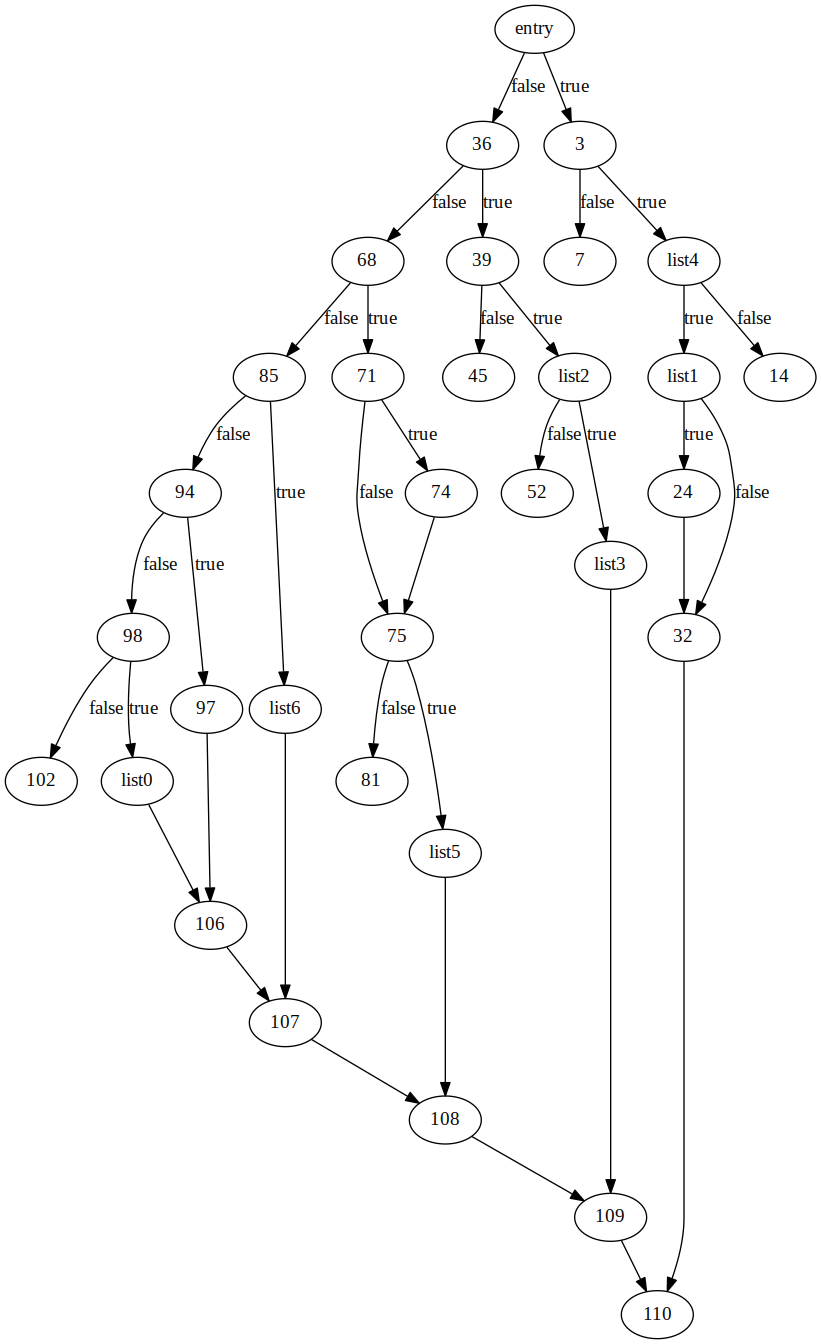
\includegraphics[width=\textwidth]{inc/appendices/control_flow_analysis_example/stmt_2.png}
	\end{subfigure}
	\caption{\textbf{Step 2}. The CFG from \textbf{step 1} (left) and a simplified CFG (right) after identifying consecutive statements (see figure \ref{fig:list_graph_representation}).}
	\label{fig:step_2}
\end{figure}

% if
\begin{figure}[htbp]
	\centering
	\begin{subfigure}[ht]{0.45\textwidth}
		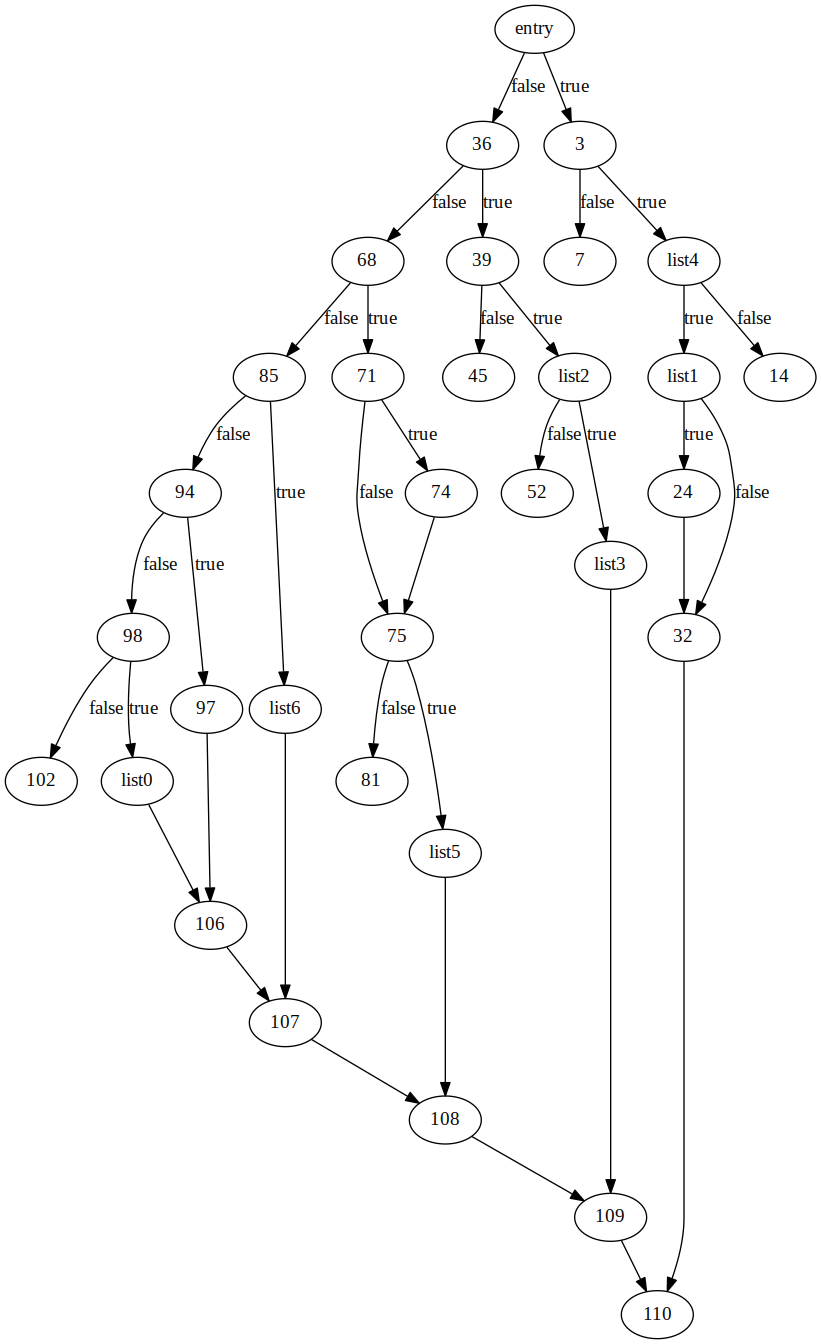
\includegraphics[width=\textwidth]{inc/appendices/control_flow_analysis_example/stmt_2.png}
	\end{subfigure}
	\qquad
	\begin{subfigure}[ht]{0.45\textwidth}
		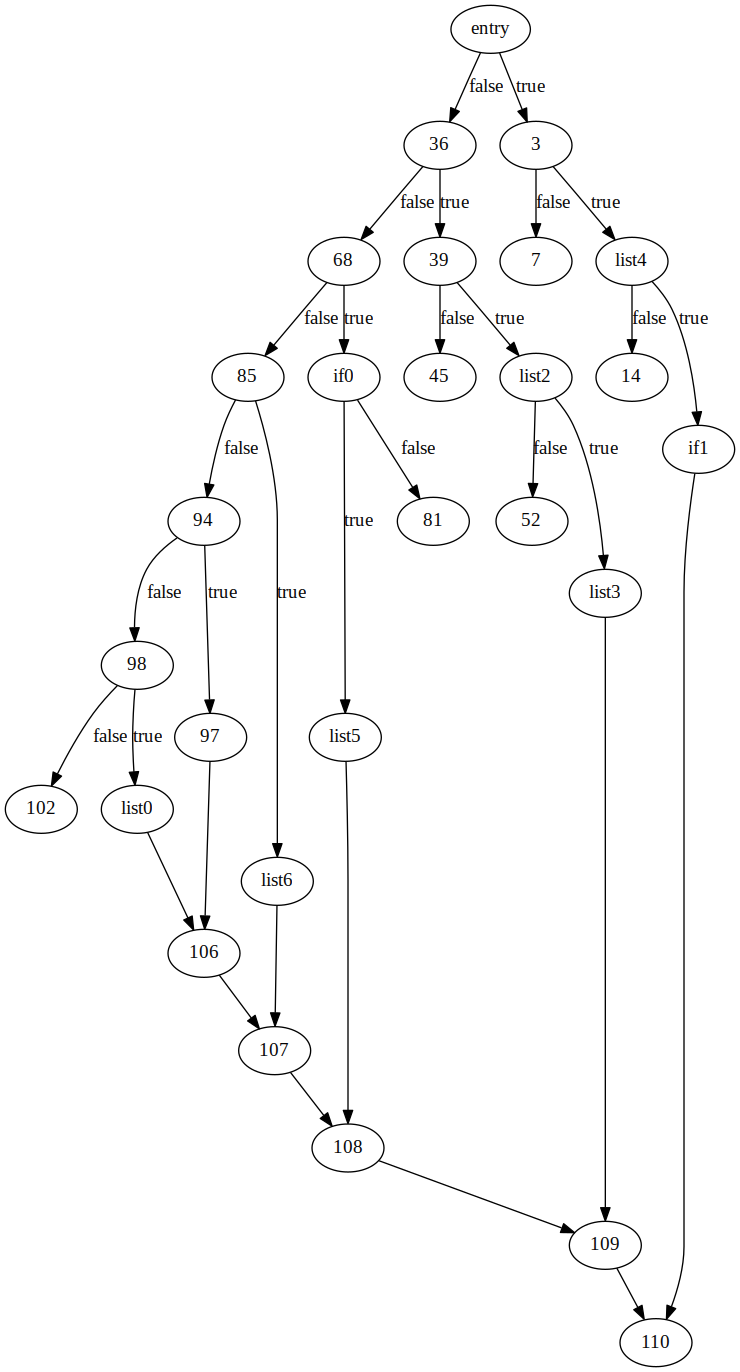
\includegraphics[width=\textwidth]{inc/appendices/control_flow_analysis_example/stmt_3.png}
	\end{subfigure}
	\caption{\textbf{Step 3}. The CFG from \textbf{step 2} (left) and a simplified CFG (right) after identifying 1-way conditionals (see figure \ref{fig:if_graph_representation}).}
	\label{fig:step_3}
\end{figure}

% if_return
\begin{figure}[htbp]
	\centering
	\begin{subfigure}[ht]{0.45\textwidth}
		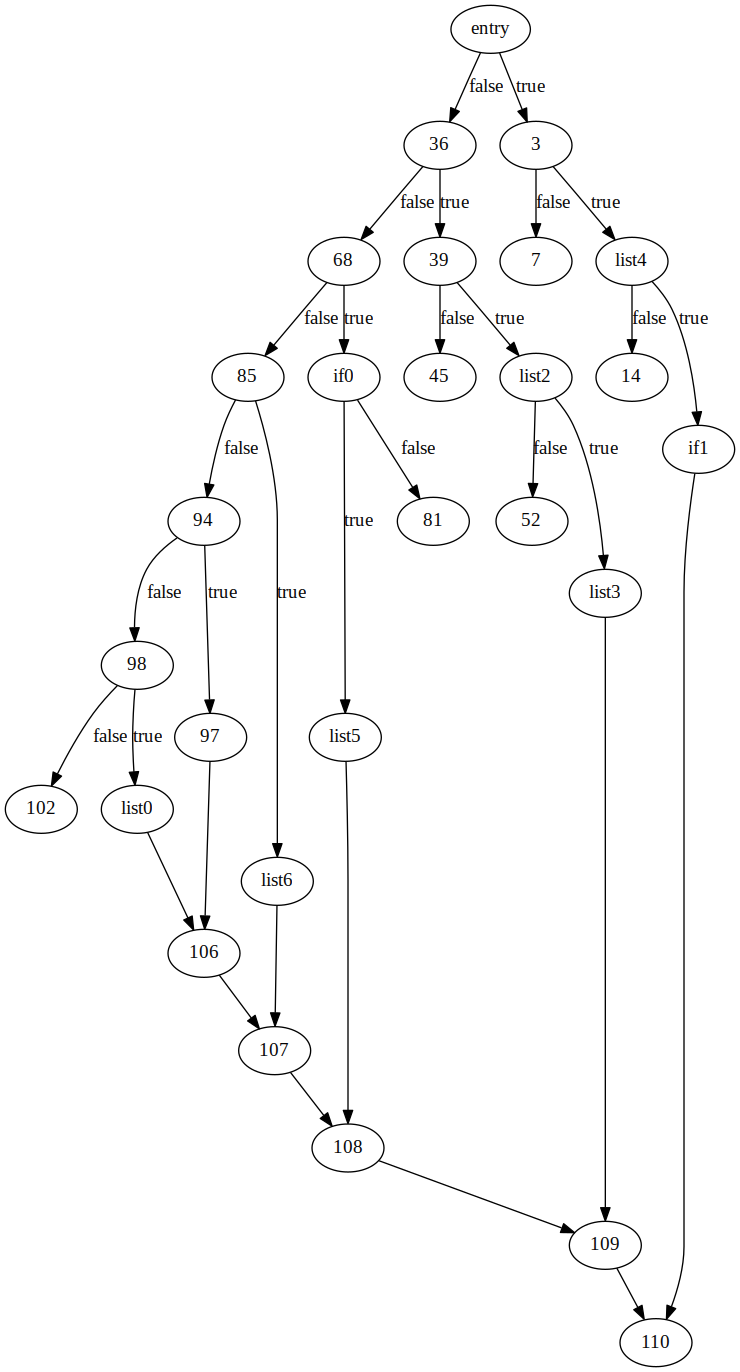
\includegraphics[width=\textwidth]{inc/appendices/control_flow_analysis_example/stmt_3.png}
	\end{subfigure}
	\qquad
	\begin{subfigure}[ht]{0.45\textwidth}
		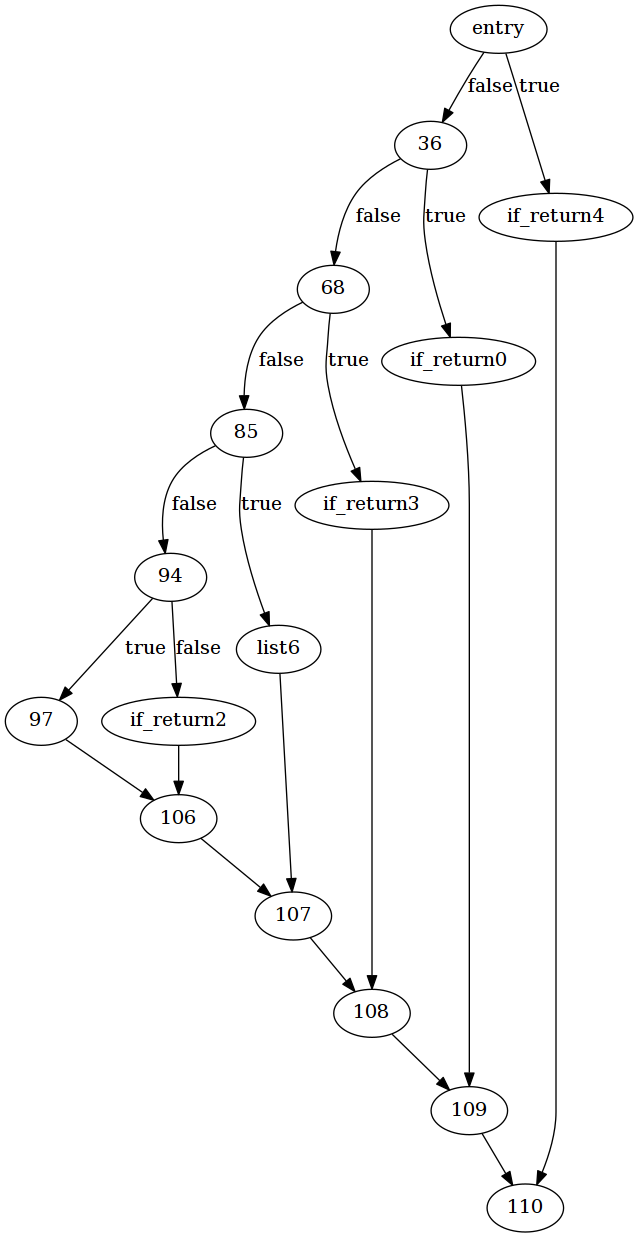
\includegraphics[width=\textwidth]{inc/appendices/control_flow_analysis_example/stmt_4.png}
	\end{subfigure}
	\caption{\textbf{Step 4}. The CFG from \textbf{step 3} (left) and a simplified CFG (right) after identifying 1-way conditionals with body return statements (see figure \ref{fig:if_return_graph_representation}).}
	\label{fig:step_4}
\end{figure}

% if_else
\begin{figure}[htbp]
	\centering
	\begin{subfigure}[ht]{0.45\textwidth}
		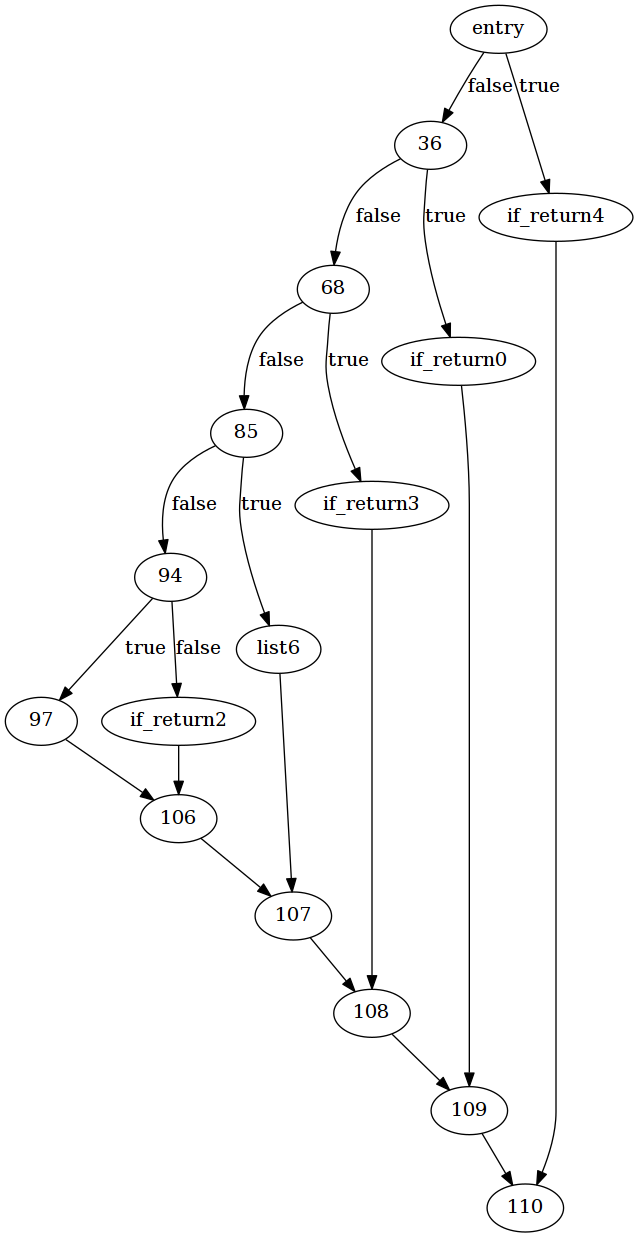
\includegraphics[width=\textwidth]{inc/appendices/control_flow_analysis_example/stmt_4.png}
	\end{subfigure}
	\qquad
	\begin{subfigure}[ht]{0.45\textwidth}
		\centering
		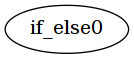
\includegraphics[width=0.3\textwidth]{inc/appendices/control_flow_analysis_example/stmt_5.png}
	\end{subfigure}
	\caption{\textbf{Step 5}. The CFG from \textbf{step 4} (left) and a simplified CFG (right) after identifying 2-way conditionals (see figure \ref{fig:if_else_graph_representation}).}
	\label{fig:step_5}
\end{figure}
